\documentclass{article}

\usepackage[final]{nips_2017}
\usepackage[utf8]{inputenc} % allow utf-8 input
\usepackage[T1]{fontenc}    % use 8-bit T1 fonts
\usepackage{hyperref}       % hyperlinks
\usepackage{url}            % simple URL typesetting
\usepackage{booktabs}       % professional-quality tables
\usepackage{amsfonts}       % blackboard math symbols
\usepackage{nicefrac}       % compact symbols for 1/2, etc.
\usepackage{microtype}      % microtypography
\usepackage{graphicx}
\usepackage{enumerate}
\usepackage{colonequals}

\newcommand{\vect}[1]{\mathbf{#1}}
\newcommand{\defas}{\colonequals}
\newcommand{\abs}[1]{\left|#1\right|}
\newcommand{\paren}[1]{\left(#1\right)}
\newcommand{\argmin}{\mathop{\mathrm{argmin}}}
\newcommand{\trans}[1]{{#1}^\mathrm{T}}


\title{Kinship Verification with an Optimal CNN}

% The \author macro works with any number of authors. There are two
% commands used to separate the names and addresses of multiple
% authors: \And and \AND.
%
% Using \And between authors leaves it to LaTeX to determine where to
% break the lines. Using \AND forces a line break at that point. So,
% if LaTeX puts 3 of 4 authors names on the first line, and the last
% on the second line, try using \AND instead of \And before the third
% author name.

\author{
  Xiaowei Chu \\
  1633568 \\
  \texttt{xchu1@ucsc.edu} \\
  \And
  Zehui Cheng \\
  1633465 \\
  \texttt{zecheng@ucsc.edu} \\
  \And
  Jianfeng Zhao \\
  1633705 \\
  \texttt{zhao65@ucsc.edu} \\
  \And
  Xiaoying Huang \\
  1634531 \\
  \texttt{xhuang82@ucsc.edu} \\
  \AND
  Wei-Lin Wu \\
  1634541 \\
  \texttt{wwu53@ucsc.edu} \\
}

\begin{document}
% \nipsfinalcopy is no longer used

\maketitle

\begin{abstract}
Kinship refers to the blood relationship between two people. It is known that we humans have the ability to estimate this relationship based on physiological features, especially facial characteristics. In this project, we focus on the 4 different types of parent-child kinship (father-daughter, father-son, mother-daughter, mother-son) and build a model to measure it given two face images using three different methods, and then we conduct experiments to evaluate these methods.
\end{abstract}

\section{Introduction}
\subsection{Background}
Identifying the kinship between parents and children has long been a subject. It often finds its application in divorce suits. But there are also situations where this identification might be useful: Identifying missing children that were lost at birth or in their childhood and avoiding consanguineous marriages for eugenic concerns. DNA test could be a solution, but at a high price. Moreover, both people whose kinship is to be examined need to agree for the test.

We are thus motivated to design an easy solution using machine learning: Train a model to recognize the biological relationship between people based on their facial features. According to physiology, people with genetic overlap have similar appearances, especially in their faces. Therefore, kinship verification can be implemented by examining face features with machine learning algorithms.

\subsection{Related work}
There have been researches on kinship verification, and they can be classified into three categories.

The first category is concerned with feature extraction of face images to improve the verification rate. In [1], P.\ Alirezazadeh, A.\ Fathi, and F.\ Abdali-Mohammadi propose genetic algorithms (which is based on the evolution of consecutive generations) to combine local and global features for face images. In addition, some discriminant features are selected by using genetic algorithms in order to improve the verification rate and reduce ineffective features.

The second category uses the metric learning based method. H.\ Yan, X.\ Zhou, and Y.\ Ge [2] use a new neighborhood repulsed correlation metric learning by leveraging the correlation similarity measurement (draw positive pairs near and repulse negative pairs), a more powerful strategy. The metric-based algorithm assesses kinship by calculating the similarity between different images. However, the similarity method is critical for the verification rate, and it is hard to find the best similarity method manually. Therefore, it leads to another category of kinship verification method without supervision.

The third category evaluates kinship using machine learning based algorithms, such as Convolutional Neural Network (CNN). K.\ Zhang, Y.\ Huang, C.\ Song, H.\ Wu1, L.\ Wang [3] use high-level feature extraction for facial information from neuron activations of the last hidden layer in the neurons network and then feed these features learned from neural network into a softmax classifier to identify the kinship between two people. In addition, this method considers the significance of the key point in the facial features.

\subsection{Our contribution}
The technique to recognize kinship using neural network in [3] motivated us to design the following three approaches:
\begin{enumerate}[(1)]
%
\item Feature extraction by concatenation.
%
\item Feature extraction by expansion.
%
\item Feature extraction by (deep) CNN.
%
\end{enumerate}

\section{Approaches}
In this section, we explain our approaches in details.
\subsection{Feature extraction by concatenation}  %%%%%%%%%%  1
In this approach, we formulate a triplet probability embedding learning method to train 128-dimensional features using IJB-A data set and CASIA-WebFace data set based on the idea of [4]:

To learn the embedding $\vect{W}$ from a given set of triplets $\mathbb{T}$, solve the following optimization
\[
\argmin_\vect{W} \sum^\mathbb{T}_{\vect{v}_i, \vect{v}_j, \vect{v}_k} -\log(p_{ijk})
\]
where
\[
p_{ijk} = \frac{e^{S_\vect{W}(\vect{v}_i, \vect{v}_j)}}{e^{S_\vect{W}(\vect{v}_i, \vect{v}_j)} + e^{S_\vect{W}(\vect{v}_i, \vect{v}_k)}}
\]
The gradient update for W is given as
\[
\vect{W}_{\tau + 1} = \vect{W}_\tau - \eta \ast \vect{W}_\tau \ast (1 - p_{ijk}) \ast (\vect{v}_i \trans{(\vect{v}_j - \vect{v}_k)} + (\vect{v}_j - \vect{v}_k) \trans{\vect{v}_i})
\]
Computes the embedding $\vect{W}$ based on satisfying a hinge loss constraint
\[
\argmin_\vect{W} \sum_{(\vect{v}_i, \vect{v}_j, \vect{v}_k) \in \mathbb{T}} \max \{0, \alpha + \trans({\vect{v}_i - \vect{v}_j)} \trans{\vect{W}} \vect{W} (\vect{v}_i - \vect{v}_j) - \trans{(\vect{v}_i - \vect{v}_k)} \trans{\vect{W}} \vect{W} (\vect{v}_i - \vect{v}_k) \}
\]

As for preprocessing, given two face images, we extract 128 features from each image and combine them to yield a total of 256 features where the features from the first image precede those from the second, and then we use these features to train our CNN. The person of the first image is taken as parent, while the second as child.

Finally, in addition to the input layer our CNN consists of three layers where we use different activation functions for different layers: Relu function for the first layer, logistic function for the second layer, and softmax function for the third layer. (See Figure 1).
\begin{figure}[h]
  \centering
  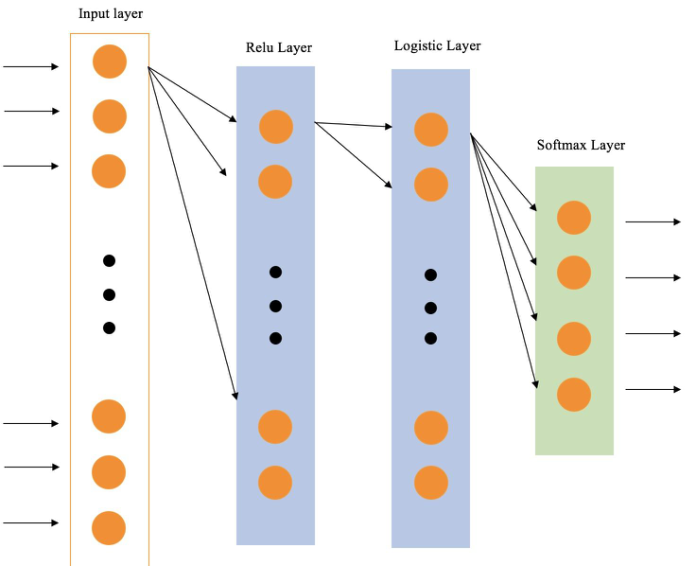
\includegraphics[width=8cm]{CNN_1.png}
  %\fbox{\rule[-.5cm]{0cm}{4cm} \rule[-.5cm]{4cm}{0cm}}
  \caption{CNN used in the first and second approaches.}
\end{figure}

\subsection{Feature extraction by expansion} %%%%%%%%%%  2
This approach is identical to the first approach except that after extracting 128 features from each image we expand them to yield a total of 641 features; more specifically, given feature vectors $\vect{x} = (x_1, \ldots, x_{128})$ and $\vect{y} = (y_1, \ldots, y_{128})$ from the two images, we expand them to give the 641-dimensional feature vector $\vect{z}$ such that it consists of the 128 vectors
\[
\vect{z}_i = \paren{x_i, y_i, \frac{x_i + y_i}{2}, 10x_iy_i, x_i - y_i}, \  1 \leq i \leq 128
\]
in sequential order, followed by the Euclidean distance
\[
\abs{\vect{x} - \vect{y}} \defas \sqrt{\sum^{128}_{i = 1} (x_i - y_i)^2}
\]
of $\vect{x}$ and $\vect{y}$.

\subsection{Feature extraction by (deep) CNN} %%%%%%%%%%  3
In this final approach, we use 4-layer CNN to extract 512 features from each of the two images and then feed these features for the next 2-layer CNN to learn. See the figure below:
\begin{figure}[h]
  \centering
  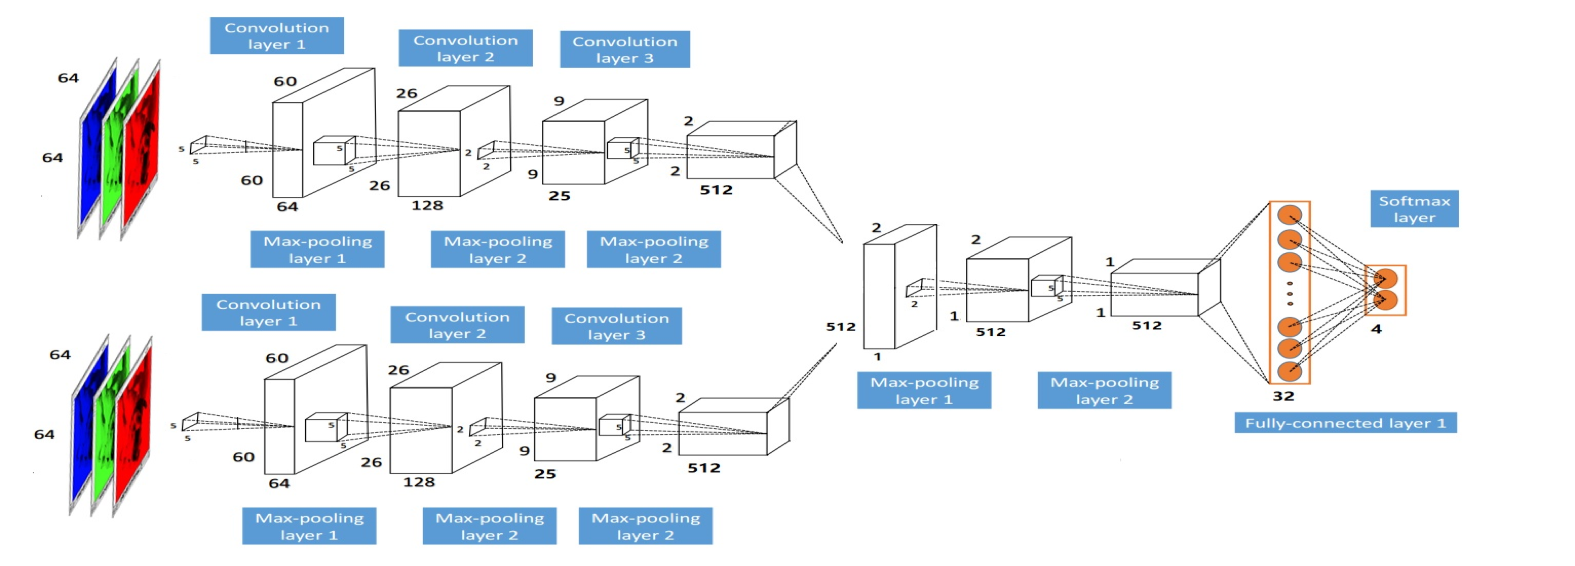
\includegraphics[width=12cm]{CNN_2.png}
  %\fbox{\rule[-.5cm]{0cm}{4cm} \rule[-.5cm]{4cm}{0cm}}
  \caption{Visualization of the third approach.}
\end{figure}

\section{Experiment and analysis}
To conduct our experiment, we use the total 8000 pairs of parent-child face images from SmileFIW (4000 pairs for each type of parent-child kinship) as our train data set and the total 1190 pairs of parent-child face images from KinFaceW (roughly 300 pairs for each type) as the test data set.

Analyze the advantages/disadvantage of the three different approaches:
\begin{enumerate}[(1)]
%
\item This training is based on the order. It requires an order of input pictures in the test. For example, we must input the father’s picture at first in father-child relationship testing. And this is equivalent to making a judgment in advance.


\end{enumerate}

\section{Conclusion}
Application Scenarios:
1) Group Membership Prediction.
2) Family Album Organization on mobile phones.
3) Social Network Relation Detection.
4) Social Media Analysis
5) Facilitate Genealogical Research

\section*{References}
[1] (Genetic) A Genetic Algorithm-Based Feature Selection for Kinship Verification

[2] (Metric) Neighborhood Repulsed Correlation Metric Learning for Kinship Verification

[3] (Machine Learning, CNN) Kinship Verification with Deep Convolutional Neural Networks

[4] (TPE) Triplet Probabilistic Embedding for Face Verification and Clustering

\end{document}